% Options for packages loaded elsewhere
\PassOptionsToPackage{unicode}{hyperref}
\PassOptionsToPackage{hyphens}{url}
%
\documentclass[
]{article}
\usepackage{lmodern}
\usepackage{amssymb,amsmath}
\usepackage{ifxetex,ifluatex}
\ifnum 0\ifxetex 1\fi\ifluatex 1\fi=0 % if pdftex
  \usepackage[T1]{fontenc}
  \usepackage[utf8]{inputenc}
  \usepackage{textcomp} % provide euro and other symbols
\else % if luatex or xetex
  \usepackage{unicode-math}
  \defaultfontfeatures{Scale=MatchLowercase}
  \defaultfontfeatures[\rmfamily]{Ligatures=TeX,Scale=1}
\fi
% Use upquote if available, for straight quotes in verbatim environments
\IfFileExists{upquote.sty}{\usepackage{upquote}}{}
\IfFileExists{microtype.sty}{% use microtype if available
  \usepackage[]{microtype}
  \UseMicrotypeSet[protrusion]{basicmath} % disable protrusion for tt fonts
}{}
\makeatletter
\@ifundefined{KOMAClassName}{% if non-KOMA class
  \IfFileExists{parskip.sty}{%
    \usepackage{parskip}
  }{% else
    \setlength{\parindent}{0pt}
    \setlength{\parskip}{6pt plus 2pt minus 1pt}}
}{% if KOMA class
  \KOMAoptions{parskip=half}}
\makeatother
\usepackage{xcolor}
\IfFileExists{xurl.sty}{\usepackage{xurl}}{} % add URL line breaks if available
\IfFileExists{bookmark.sty}{\usepackage{bookmark}}{\usepackage{hyperref}}
\hypersetup{
  pdftitle={Task-1 Linear Regression},
  hidelinks,
  pdfcreator={LaTeX via pandoc}}
\urlstyle{same} % disable monospaced font for URLs
\usepackage[margin=1in]{geometry}
\usepackage{color}
\usepackage{fancyvrb}
\newcommand{\VerbBar}{|}
\newcommand{\VERB}{\Verb[commandchars=\\\{\}]}
\DefineVerbatimEnvironment{Highlighting}{Verbatim}{commandchars=\\\{\}}
% Add ',fontsize=\small' for more characters per line
\usepackage{framed}
\definecolor{shadecolor}{RGB}{248,248,248}
\newenvironment{Shaded}{\begin{snugshade}}{\end{snugshade}}
\newcommand{\AlertTok}[1]{\textcolor[rgb]{0.94,0.16,0.16}{#1}}
\newcommand{\AnnotationTok}[1]{\textcolor[rgb]{0.56,0.35,0.01}{\textbf{\textit{#1}}}}
\newcommand{\AttributeTok}[1]{\textcolor[rgb]{0.77,0.63,0.00}{#1}}
\newcommand{\BaseNTok}[1]{\textcolor[rgb]{0.00,0.00,0.81}{#1}}
\newcommand{\BuiltInTok}[1]{#1}
\newcommand{\CharTok}[1]{\textcolor[rgb]{0.31,0.60,0.02}{#1}}
\newcommand{\CommentTok}[1]{\textcolor[rgb]{0.56,0.35,0.01}{\textit{#1}}}
\newcommand{\CommentVarTok}[1]{\textcolor[rgb]{0.56,0.35,0.01}{\textbf{\textit{#1}}}}
\newcommand{\ConstantTok}[1]{\textcolor[rgb]{0.00,0.00,0.00}{#1}}
\newcommand{\ControlFlowTok}[1]{\textcolor[rgb]{0.13,0.29,0.53}{\textbf{#1}}}
\newcommand{\DataTypeTok}[1]{\textcolor[rgb]{0.13,0.29,0.53}{#1}}
\newcommand{\DecValTok}[1]{\textcolor[rgb]{0.00,0.00,0.81}{#1}}
\newcommand{\DocumentationTok}[1]{\textcolor[rgb]{0.56,0.35,0.01}{\textbf{\textit{#1}}}}
\newcommand{\ErrorTok}[1]{\textcolor[rgb]{0.64,0.00,0.00}{\textbf{#1}}}
\newcommand{\ExtensionTok}[1]{#1}
\newcommand{\FloatTok}[1]{\textcolor[rgb]{0.00,0.00,0.81}{#1}}
\newcommand{\FunctionTok}[1]{\textcolor[rgb]{0.00,0.00,0.00}{#1}}
\newcommand{\ImportTok}[1]{#1}
\newcommand{\InformationTok}[1]{\textcolor[rgb]{0.56,0.35,0.01}{\textbf{\textit{#1}}}}
\newcommand{\KeywordTok}[1]{\textcolor[rgb]{0.13,0.29,0.53}{\textbf{#1}}}
\newcommand{\NormalTok}[1]{#1}
\newcommand{\OperatorTok}[1]{\textcolor[rgb]{0.81,0.36,0.00}{\textbf{#1}}}
\newcommand{\OtherTok}[1]{\textcolor[rgb]{0.56,0.35,0.01}{#1}}
\newcommand{\PreprocessorTok}[1]{\textcolor[rgb]{0.56,0.35,0.01}{\textit{#1}}}
\newcommand{\RegionMarkerTok}[1]{#1}
\newcommand{\SpecialCharTok}[1]{\textcolor[rgb]{0.00,0.00,0.00}{#1}}
\newcommand{\SpecialStringTok}[1]{\textcolor[rgb]{0.31,0.60,0.02}{#1}}
\newcommand{\StringTok}[1]{\textcolor[rgb]{0.31,0.60,0.02}{#1}}
\newcommand{\VariableTok}[1]{\textcolor[rgb]{0.00,0.00,0.00}{#1}}
\newcommand{\VerbatimStringTok}[1]{\textcolor[rgb]{0.31,0.60,0.02}{#1}}
\newcommand{\WarningTok}[1]{\textcolor[rgb]{0.56,0.35,0.01}{\textbf{\textit{#1}}}}
\usepackage{graphicx,grffile}
\makeatletter
\def\maxwidth{\ifdim\Gin@nat@width>\linewidth\linewidth\else\Gin@nat@width\fi}
\def\maxheight{\ifdim\Gin@nat@height>\textheight\textheight\else\Gin@nat@height\fi}
\makeatother
% Scale images if necessary, so that they will not overflow the page
% margins by default, and it is still possible to overwrite the defaults
% using explicit options in \includegraphics[width, height, ...]{}
\setkeys{Gin}{width=\maxwidth,height=\maxheight,keepaspectratio}
% Set default figure placement to htbp
\makeatletter
\def\fps@figure{htbp}
\makeatother
\setlength{\emergencystretch}{3em} % prevent overfull lines
\providecommand{\tightlist}{%
  \setlength{\itemsep}{0pt}\setlength{\parskip}{0pt}}
\setcounter{secnumdepth}{-\maxdimen} % remove section numbering

\title{Task-1 Linear Regression}
\author{}
\date{\vspace{-2.5em}}

\begin{document}
\maketitle

\hypertarget{author--shivam-khandelwal}{%
\subsection{Author- Shivam Khandelwal}\label{author--shivam-khandelwal}}

\hypertarget{from-the-given-student-scores-dataset-we-need-to-make-a-linear-regression-model-and-predict-the-score-for-the-student-when-number-of-study-hours-9.25.}{%
\subsubsection{From the Given Student Scores Dataset, we need to make a
Linear Regression model and predict the score for the student when
Number of study hours=
9.25.}\label{from-the-given-student-scores-dataset-we-need-to-make-a-linear-regression-model-and-predict-the-score-for-the-student-when-number-of-study-hours-9.25.}}

\hypertarget{importing-required-libraries}{%
\paragraph{Importing Required
Libraries:}\label{importing-required-libraries}}

\begin{Shaded}
\begin{Highlighting}[]
\KeywordTok{library}\NormalTok{(ggplot2)}
\end{Highlighting}
\end{Shaded}

\begin{verbatim}
## Warning: package 'ggplot2' was built under R version 3.6.3
\end{verbatim}

\hypertarget{loading-the-dataset}{%
\paragraph{Loading the Dataset}\label{loading-the-dataset}}

\begin{Shaded}
\begin{Highlighting}[]
\NormalTok{df<-}\StringTok{ }\KeywordTok{read.csv}\NormalTok{(}\StringTok{"StudentData.csv"}\NormalTok{)}
\end{Highlighting}
\end{Shaded}

\hypertarget{summarizing-the-dataset}{%
\paragraph{Summarizing the Dataset}\label{summarizing-the-dataset}}

\begin{Shaded}
\begin{Highlighting}[]
\KeywordTok{head}\NormalTok{(df, }\DataTypeTok{n=}\DecValTok{10}\NormalTok{)}
\end{Highlighting}
\end{Shaded}

\begin{verbatim}
##    Hours Scores
## 1    2.5     21
## 2    5.1     47
## 3    3.2     27
## 4    8.5     75
## 5    3.5     30
## 6    1.5     20
## 7    9.2     88
## 8    5.5     60
## 9    8.3     81
## 10   2.7     25
\end{verbatim}

\begin{Shaded}
\begin{Highlighting}[]
\KeywordTok{summary}\NormalTok{(df)}
\end{Highlighting}
\end{Shaded}

\begin{verbatim}
##      Hours           Scores     
##  Min.   :1.100   Min.   :17.00  
##  1st Qu.:2.700   1st Qu.:30.00  
##  Median :4.800   Median :47.00  
##  Mean   :5.012   Mean   :51.48  
##  3rd Qu.:7.400   3rd Qu.:75.00  
##  Max.   :9.200   Max.   :95.00
\end{verbatim}

\hypertarget{visualizing-the-data-of-scores-w.r.t.-hours}{%
\paragraph{Visualizing the Data of Scores w.r.t.
Hours}\label{visualizing-the-data-of-scores-w.r.t.-hours}}

\begin{Shaded}
\begin{Highlighting}[]
\KeywordTok{ggplot}\NormalTok{(df, }\KeywordTok{aes}\NormalTok{(}\DataTypeTok{x=}\NormalTok{Hours, }\DataTypeTok{y=}\NormalTok{Scores)) }\OperatorTok{+}\StringTok{ }
\StringTok{  }\KeywordTok{geom_point}\NormalTok{()}
\end{Highlighting}
\end{Shaded}

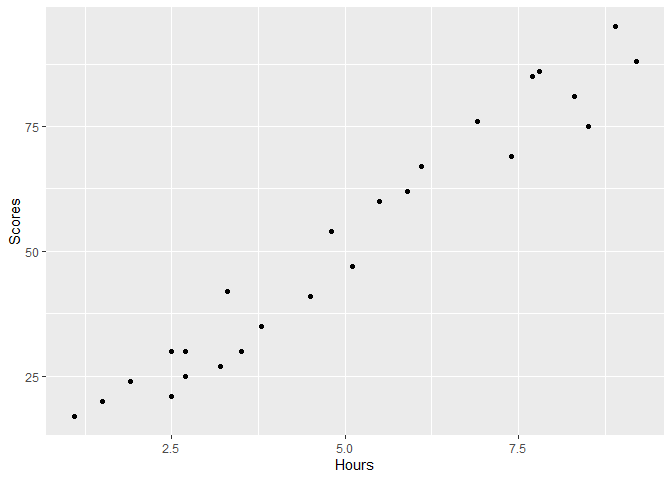
\includegraphics{Task1LinearRegression_files/figure-latex/unnamed-chunk-3-1.pdf}

\hypertarget{checking-the-level-of-correlation}{%
\paragraph{Checking the level of
correlation}\label{checking-the-level-of-correlation}}

\begin{Shaded}
\begin{Highlighting}[]
\KeywordTok{cor}\NormalTok{(df}\OperatorTok{$}\NormalTok{Hours, df}\OperatorTok{$}\NormalTok{Scores)}
\end{Highlighting}
\end{Shaded}

\begin{verbatim}
## [1] 0.9761907
\end{verbatim}

We can see there is a strong co-relation between Number of Hours a
Student Studied and Scores obtained by them.

\hypertarget{defining-a-linear-regression-model-training-on-all-of-the-dataset}{%
\paragraph{Defining a Linear Regression Model, training on all of the
dataset}\label{defining-a-linear-regression-model-training-on-all-of-the-dataset}}

\begin{Shaded}
\begin{Highlighting}[]
\NormalTok{LinearReg <-}\StringTok{ }\KeywordTok{lm}\NormalTok{(Scores }\OperatorTok{~}\StringTok{ }\NormalTok{Hours, }\DataTypeTok{data=}\NormalTok{df)  }
\KeywordTok{print}\NormalTok{(LinearReg)}
\end{Highlighting}
\end{Shaded}

\begin{verbatim}
## 
## Call:
## lm(formula = Scores ~ Hours, data = df)
## 
## Coefficients:
## (Intercept)        Hours  
##       2.484        9.776
\end{verbatim}

\hypertarget{summarizing-the-linear-regression-model}{%
\paragraph{Summarizing the Linear Regression
Model}\label{summarizing-the-linear-regression-model}}

\begin{Shaded}
\begin{Highlighting}[]
\KeywordTok{summary}\NormalTok{(LinearReg)}
\end{Highlighting}
\end{Shaded}

\begin{verbatim}
## 
## Call:
## lm(formula = Scores ~ Hours, data = df)
## 
## Residuals:
##     Min      1Q  Median      3Q     Max 
## -10.578  -5.340   1.839   4.593   7.265 
## 
## Coefficients:
##             Estimate Std. Error t value Pr(>|t|)    
## (Intercept)   2.4837     2.5317   0.981    0.337    
## Hours         9.7758     0.4529  21.583   <2e-16 ***
## ---
## Signif. codes:  0 '***' 0.001 '**' 0.01 '*' 0.05 '.' 0.1 ' ' 1
## 
## Residual standard error: 5.603 on 23 degrees of freedom
## Multiple R-squared:  0.9529, Adjusted R-squared:  0.9509 
## F-statistic: 465.8 on 1 and 23 DF,  p-value: < 2.2e-16
\end{verbatim}

The model is statistically significant as p-value is smaller than 0.05
(p value: \textless{} 2.2e-16), and the p-value (\textless2e-16) for the
predictor variable is also smaller

\hypertarget{visualizing-the-regression-line}{%
\paragraph{Visualizing the Regression
line}\label{visualizing-the-regression-line}}

\begin{Shaded}
\begin{Highlighting}[]
\KeywordTok{ggplot}\NormalTok{(df, }\KeywordTok{aes}\NormalTok{(}\DataTypeTok{x=}\NormalTok{Hours, }\DataTypeTok{y=}\NormalTok{Scores)) }\OperatorTok{+}\StringTok{ }
\StringTok{  }\KeywordTok{geom_point}\NormalTok{()}\OperatorTok{+}\KeywordTok{stat_smooth}\NormalTok{(}\DataTypeTok{method =}\NormalTok{ lm)}
\end{Highlighting}
\end{Shaded}

\begin{verbatim}
## `geom_smooth()` using formula 'y ~ x'
\end{verbatim}

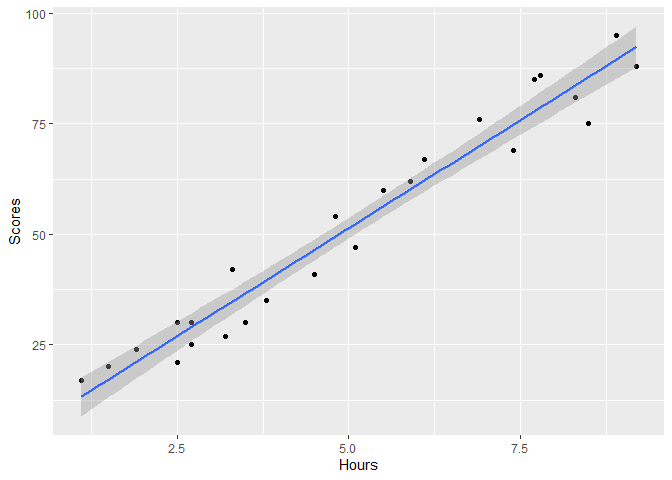
\includegraphics{Task1LinearRegression_files/figure-latex/unnamed-chunk-7-1.pdf}
\#\#\#\# Next looking for confidence interval for the model:

\begin{Shaded}
\begin{Highlighting}[]
\KeywordTok{confint}\NormalTok{(LinearReg)}
\end{Highlighting}
\end{Shaded}

\begin{verbatim}
##                 2.5 %    97.5 %
## (Intercept) -2.753470  7.720817
## Hours        8.838823 10.712784
\end{verbatim}

\hypertarget{predicting-the-score-when-study-hours9.25}{%
\paragraph{Predicting the Score when study
Hours=9.25}\label{predicting-the-score-when-study-hours9.25}}

\begin{Shaded}
\begin{Highlighting}[]
\NormalTok{ScorePred <-}\StringTok{ }\KeywordTok{predict}\NormalTok{(LinearReg, }\KeywordTok{data.frame}\NormalTok{(}\DataTypeTok{Hours =} \KeywordTok{c}\NormalTok{(}\FloatTok{9.25}\NormalTok{)))}
\NormalTok{ScorePred}
\end{Highlighting}
\end{Shaded}

\begin{verbatim}
##        1 
## 92.90985
\end{verbatim}

\end{document}
